\section{文の属性による定義}
\label{sec_attr}
本章では，お題文ありを直接付与する代わりに，画像から観測できる文の属性を付与し，お題文ありを属性から規則で導く定義を提案する．
提案の定義では，誰が書いたか，題のつもりで書いたか，既存の歌詞や台詞の引用であるかを記録しない．

\subsection{文字の層}
文字の層は，画像中の読める文字がどこにどう書かれているかを表す複数選択の属性である．
場面の文字は，写っている世界の中にある文字であり，看板，商品の表示，本の表紙，スクリーンショットの画面の中の文字を含む．
透かし，ロゴ，署名，ボケてのテンプレートに印刷された定型の見出しも，位置によらず場面の文字とする．
吹き出しは，漫画やイラストの吹き出しと語りの枠の中の文字であり，吹き出しのない，人物の脇に描き込まれた台詞を含む．
重ねた文字は，写真や絵の上に重ねた文字であり，テレビの字幕やテロップ，写真への書き込みを含む．
元の放送の字幕か投稿者が加えたものかは問わない．
余白の文字は，写真や絵の外にある文字であり，画像の上下左右の帯や枠，無地の背景，テンプレートの文字欄に書いた文字を含む．
写真や絵の領域の上にあれば重ねた文字，外にあれば余白の文字とし，帯の下地が不透明で絵を隠している場合は余白の文字とする．
文字ありは，4つの層のどれかがある場合に真とする．

\subsection{文の形}
文の形は，重ねた文字と余白の文字について，それぞれの層にどの形の文があるかを表す複数選択の属性である．
場面の文字と吹き出しの文の形は記録しない．
空欄を含む文は，空欄を含む文と，空欄を含む文章のまとまりであり，まとまりは空欄のない文を含んでいても全体をこの形とする．
問いは疑問の形の文であり，「もし〜たら」で始まる条件の形の文を含む．
指示は回答者への依頼や命令の形の文である．
題目の句は，「〜あるある」「こんな〜は嫌だ」のように大喜利の題となる名詞句や定型の句である．
その他の文は，上記のどれでもない平叙文，台詞，題名，名前，項目の名札などである．
空欄を含む文の判定を先に行い，空欄を含むまとまりの中の問いや指示は問いや指示としない．

図\ref{fig_examples}に，層と形の例を示す．
図の記号は，層を s（場面の文字），b（吹き出し），o（重ねた文字），m（余白の文字），形を k（空欄を含む文），q（問い），i（指示），t（題目の句），x（その他の文）で表し，コロンの後に層の形を示したものである．
図\ref{fig_examples}(d)の元のアニメの字幕と，図\ref{fig_examples}(e)のテロップ風に書き加えた問いは，いずれも重ねた文字の問いとなる．

\begin{figure}[t]
    \centering
    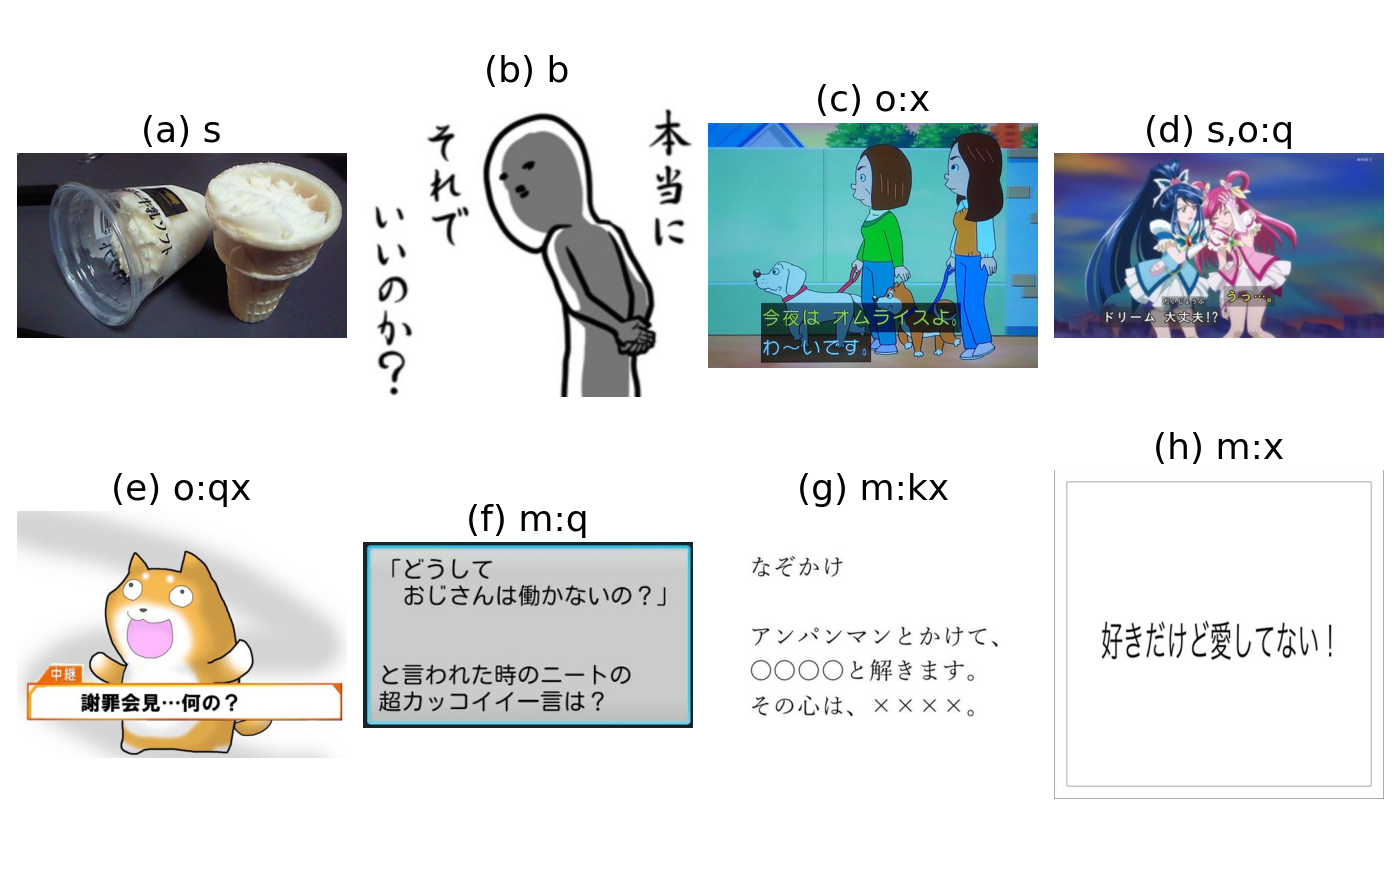
\includegraphics[width=\columnwidth]{figures/fig_examples.png}
    \caption{文の属性の例．(a) 商品の表示，(b) 人物の脇に描かれた台詞，(c) アニメの字幕の台詞，(d) アニメの字幕の問い，(e) テロップ風に書き加えた問い，(f) 枠の中の問い，(g) 名札と空欄を含む文，(h) 無地の背景の平叙文}
    \label{fig_examples}
\end{figure}

\subsection{お題文ありの規則}
重ねた文字に形 $ f $ の文がある場合に1，ない場合に0をとる変数を $ o_f $，余白の文字について同様の変数を $ m_f $ とする．
ここで $ f \in \{k, q, i, t, x\} $ は文の形の記号である．
問い，指示，題目の句のどれかが重ねた文字か余白の文字にあることを表す $ a $ を(\ref{eq_task})で定義する．

\begin{equation}
    a = \bigvee_{f \in \{q, i, t\}} \left( o_f \lor m_f \right)
    \label{eq_task}
\end{equation}

\noindent
お題文ありを導く規則として，(\ref{eq_rules})の4つを考える．

\begin{align}
    r_0 &= a, \nonumber \\
    r_1 &= a \lor m_x, \nonumber \\
    r_{1b} &= a \lor \left( m_x \land \lnot m_k \right), \nonumber \\
    r_2 &= r_1 \lor o_x
    \label{eq_rules}
\end{align}

\noindent
規則 $ r_0 $ は，問い，指示，題目の句だけを題とみなす．
規則 $ r_1 $ は，余白に書かれたその他の文も題とみなす．
余白のその他の文は，無地の背景に書いた台詞の書き出しや状況の文であることが多く，回答者はその文を読んで回答を作るためである．
規則 $ r_{1b} $ は，余白に空欄を含む文がある場合に，余白のその他の文を根拠としない．
この場合のその他の文は，名前，分類の名札，題名のように，空欄を埋めるための見出しであることが多いためである．
規則 $ r_2 $ は，重ねた文字の台詞や字幕もお題文とみなす．
本稿では $ r_{1b} $ を既定の規則とする．
規則は属性から計算するため，属性を付け直さずに規則を変更でき，規則ごとの違いを同じ目視ラベルで比べられる．

重ねた文字の問い，指示，題目の句は，$ a $ を通じて，元の字幕であるかによらずお題文ありとなる．
投稿者が写真に重ねた問いと元の字幕の問いは見た目で区別できず，どちらを除いても一方を誤るためである．
比較のため，$ a $ から重ねた文字の形を除いた規則 $ r_{1b}' = \bigvee_{f \in \{q, i, t\}} m_f \lor ( m_x \land \lnot m_k ) $ も評価する．
